\chapter{SISTAL}

En este capítulo se presenta un análisis detallado del sistema actual de gestión de uniformes corporativos, SISTAL, con el propósito de comprender su funcionamiento, estructura y alcance dentro de la organización. Se describen los principales procesos operativos, sus fortalezas, oportunidades, debilidades y amenazas mediante un análisis FODA, así como la propuesta de solución orientada a su reestructuración.
Asimismo, se incluye el diseño técnico del sistema vigente, representado a través de diagramas, los cuales permiten identificar los componentes críticos y las áreas susceptibles de mejora que fundamentan la propuesta de modernización del sistema.En este capítulo se profundizará sobre el sistema actual SISTAL, los problemas que enfrenta

\section{Análisis del Problema}

En esta sección se analizan las principales problemáticas del sistema Sistal (2008), tanto técnicas como funcionales. Se caracterizan las deficiencias que afectan la eficiencia, la escalabilidad y el mantenimiento, y se establecen los fundamentos para una mejora tecnológica.


\subsection{Situación Actual}

Sistal es una aplicación web monolítica desarrollada en PHP (2008), con base de datos MySQL sin relaciones, alojada en hosting compartido (BlueHosting) y sin control de versiones. Atiende tres actores: Administrador (empresa contratante), Funcionario (empleado) y Proveedor (confección/entrega).
Funcionalmente permite: administración de funcionarios y segmentos, captura de tallas, consolidación y envío de órdenes de confección al proveedor, seguimiento básico de estados (ingresado → confección → despacho → entrega), registro de entregas e incidencias y listados/reportes simples.

\subsubsection{Hallazgos técnicos y operativos}


\begin{itemize}
\item Arquitectura y datos: monolito acoplado; modelo de datos sin normalización, lo que limita integridad y reporting.
\item Procesos de desarrollo: sin Git ni CI/CD, sin trazabilidad de cambios ni ambientes reproducibles.
\item Infraestructura: hosting compartido con latencias e inestabilidad; sin observabilidad ni alta disponibilidad.
\item Seguridad: controles de acceso y cifrado insuficientes, sin prácticas DevSecOps.
\item UX/UI: interfaz obsoleta y no responsive; fricción en la captura de información.
\item Escalabilidad: inexistencia de multi-tenant; dificultades para servir a múltiples empresas y para integrar proveedores/logística/ERP.
\end{itemize}

\subsection{Análisis FODA}

\subsection{Solución Propuesta}

\section{Diseño del Sistema Actual}

En esta sección se documenta el diseño técnico del sistema actual, representando su estructura interna y sus principales componentes. A través de diagramas de casos de uso, base de datos, flujo, arquitectura y despliegue, se busca comprender la organización del sistema existente y las áreas que requieren modernización.


\subsection{Diagrama de Casos de Uso}

\subsection{Diagrama de Bases de Datos}

Los diagramas de base de datos presentados en las figuras \ref{fig:diagrama-bdd-1-actual} y \ref{fig:diagrama-bdd-2-actual}, son las tablas 

\begin{figure}[htbp]
    \centering
    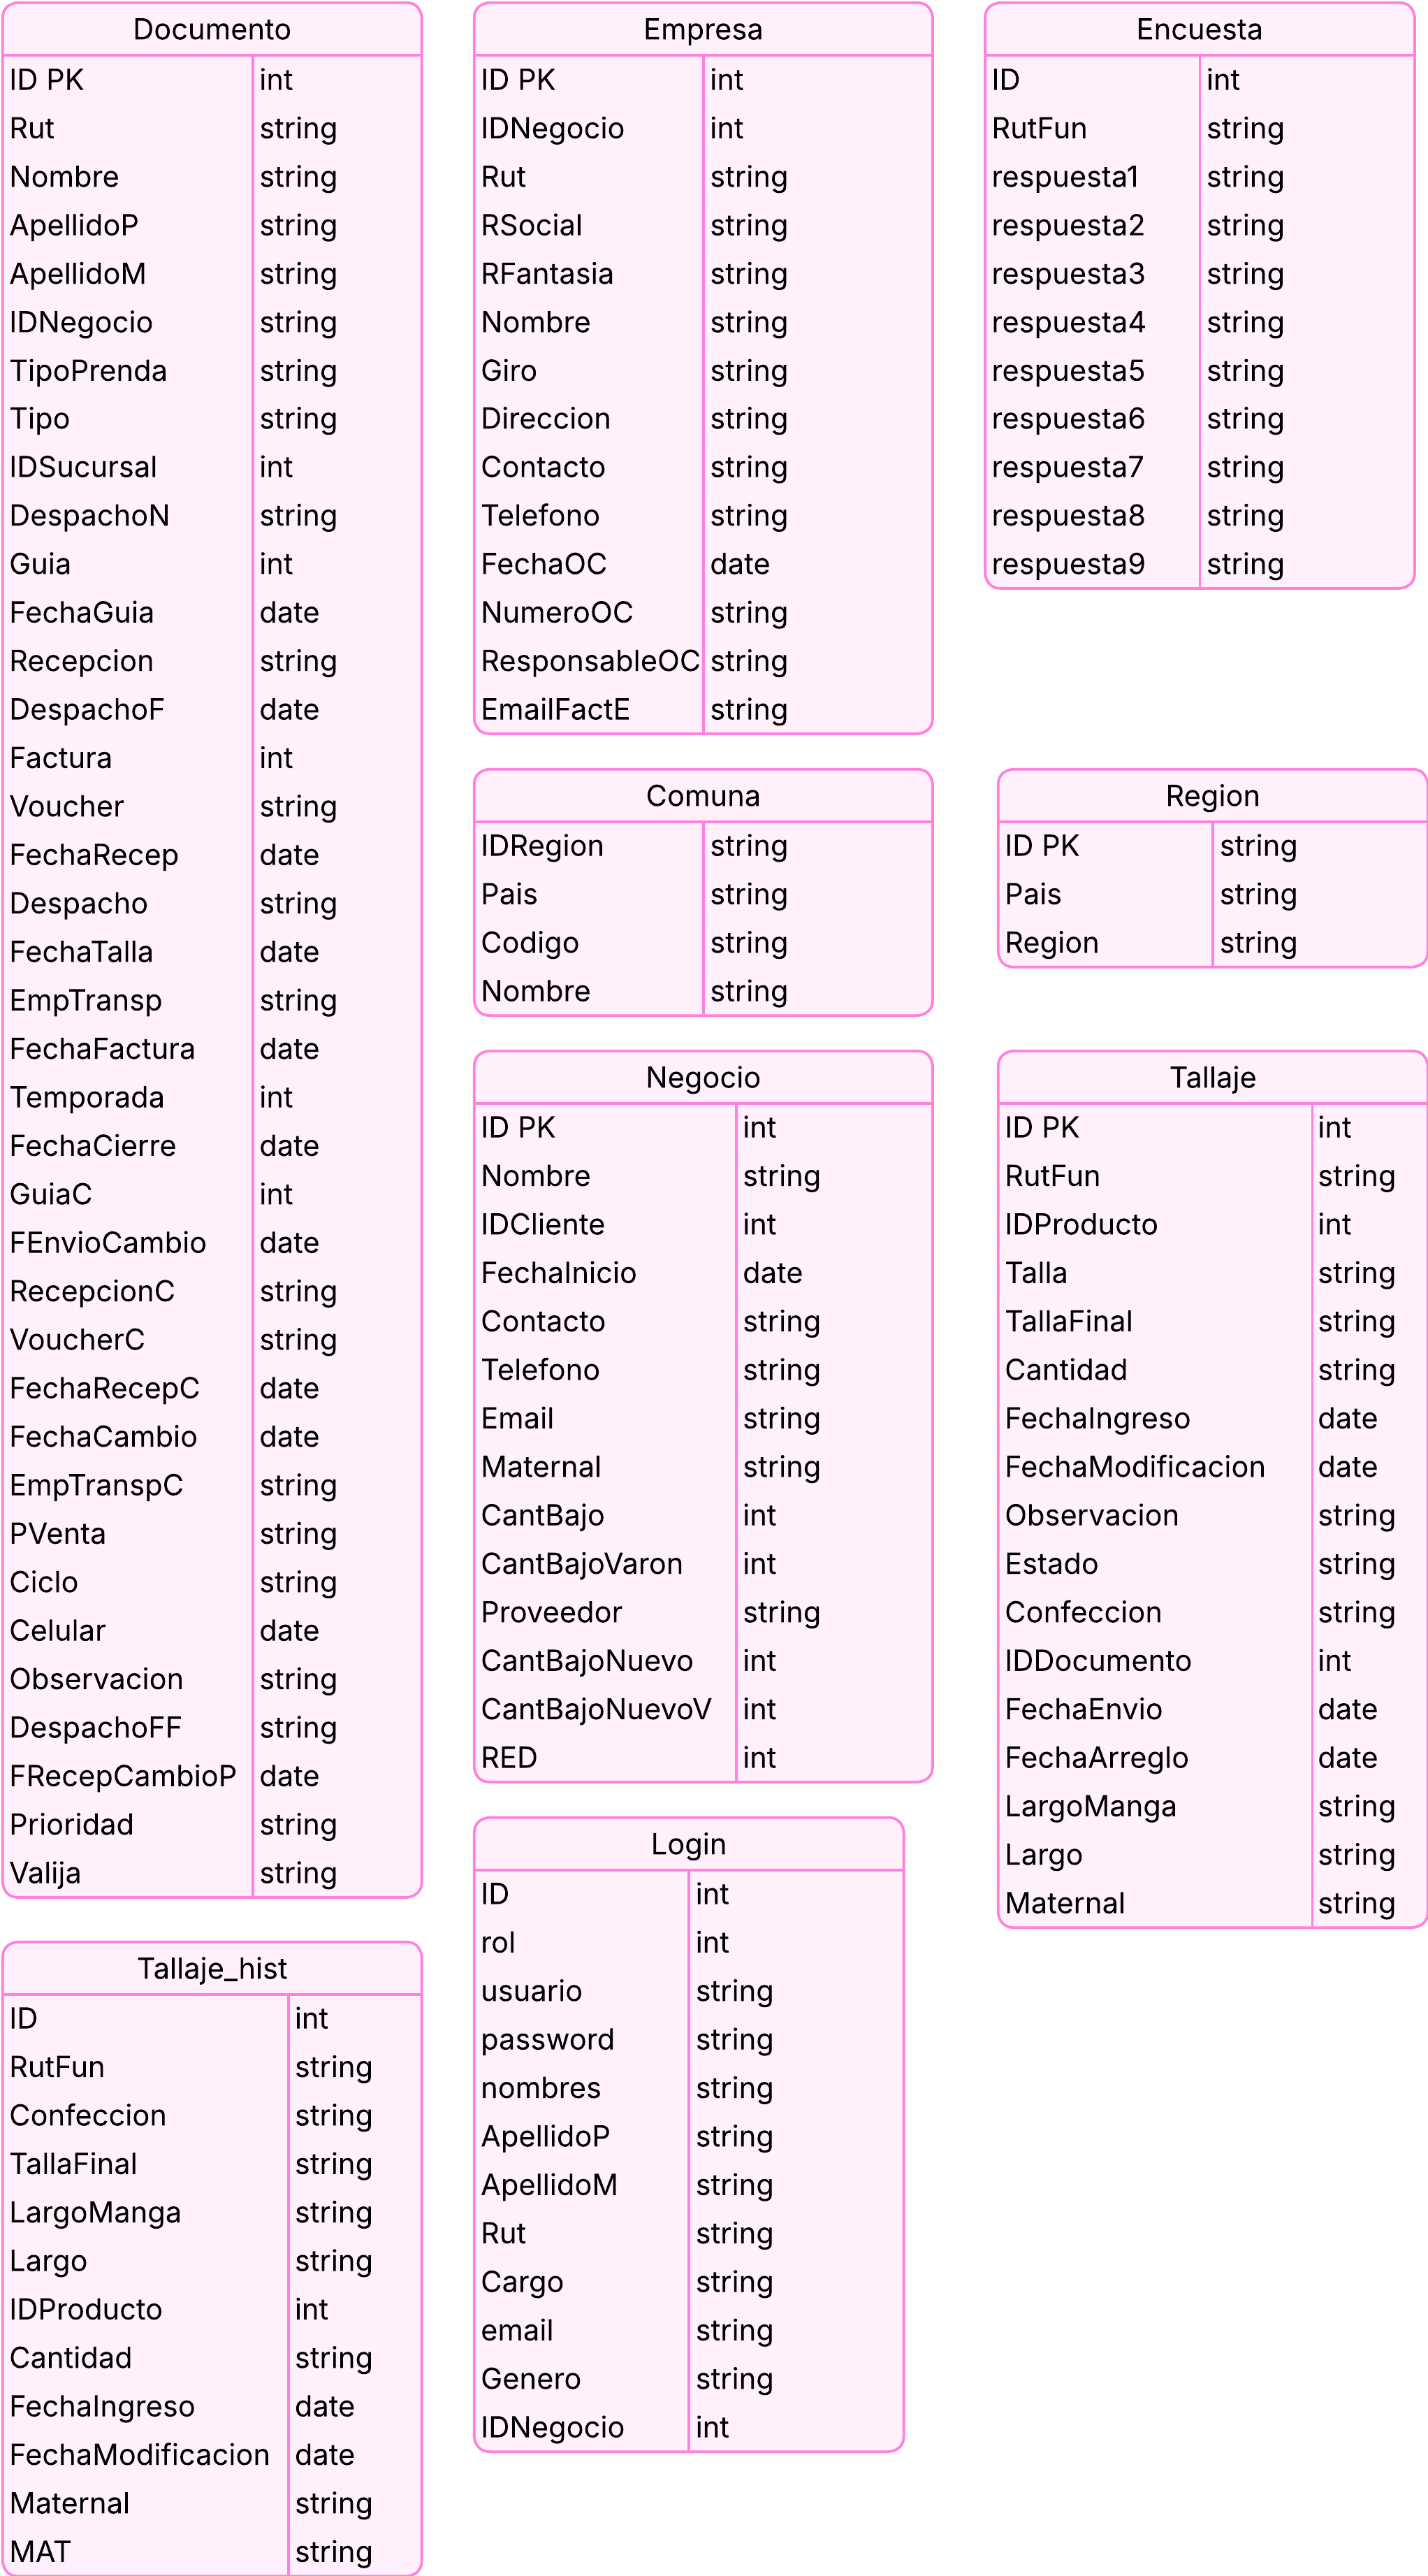
\includegraphics[height=0.9\textheight]{figuras/diagramas-actuales/diagrama-bdd-1}
    \caption{Diagrama físico de bases de datos del sistema actual (Parte 1)}
    \label{fig:diagrama-bdd-1-actual}
\end{figure}

\begin{figure}[htbp]
    \centering
    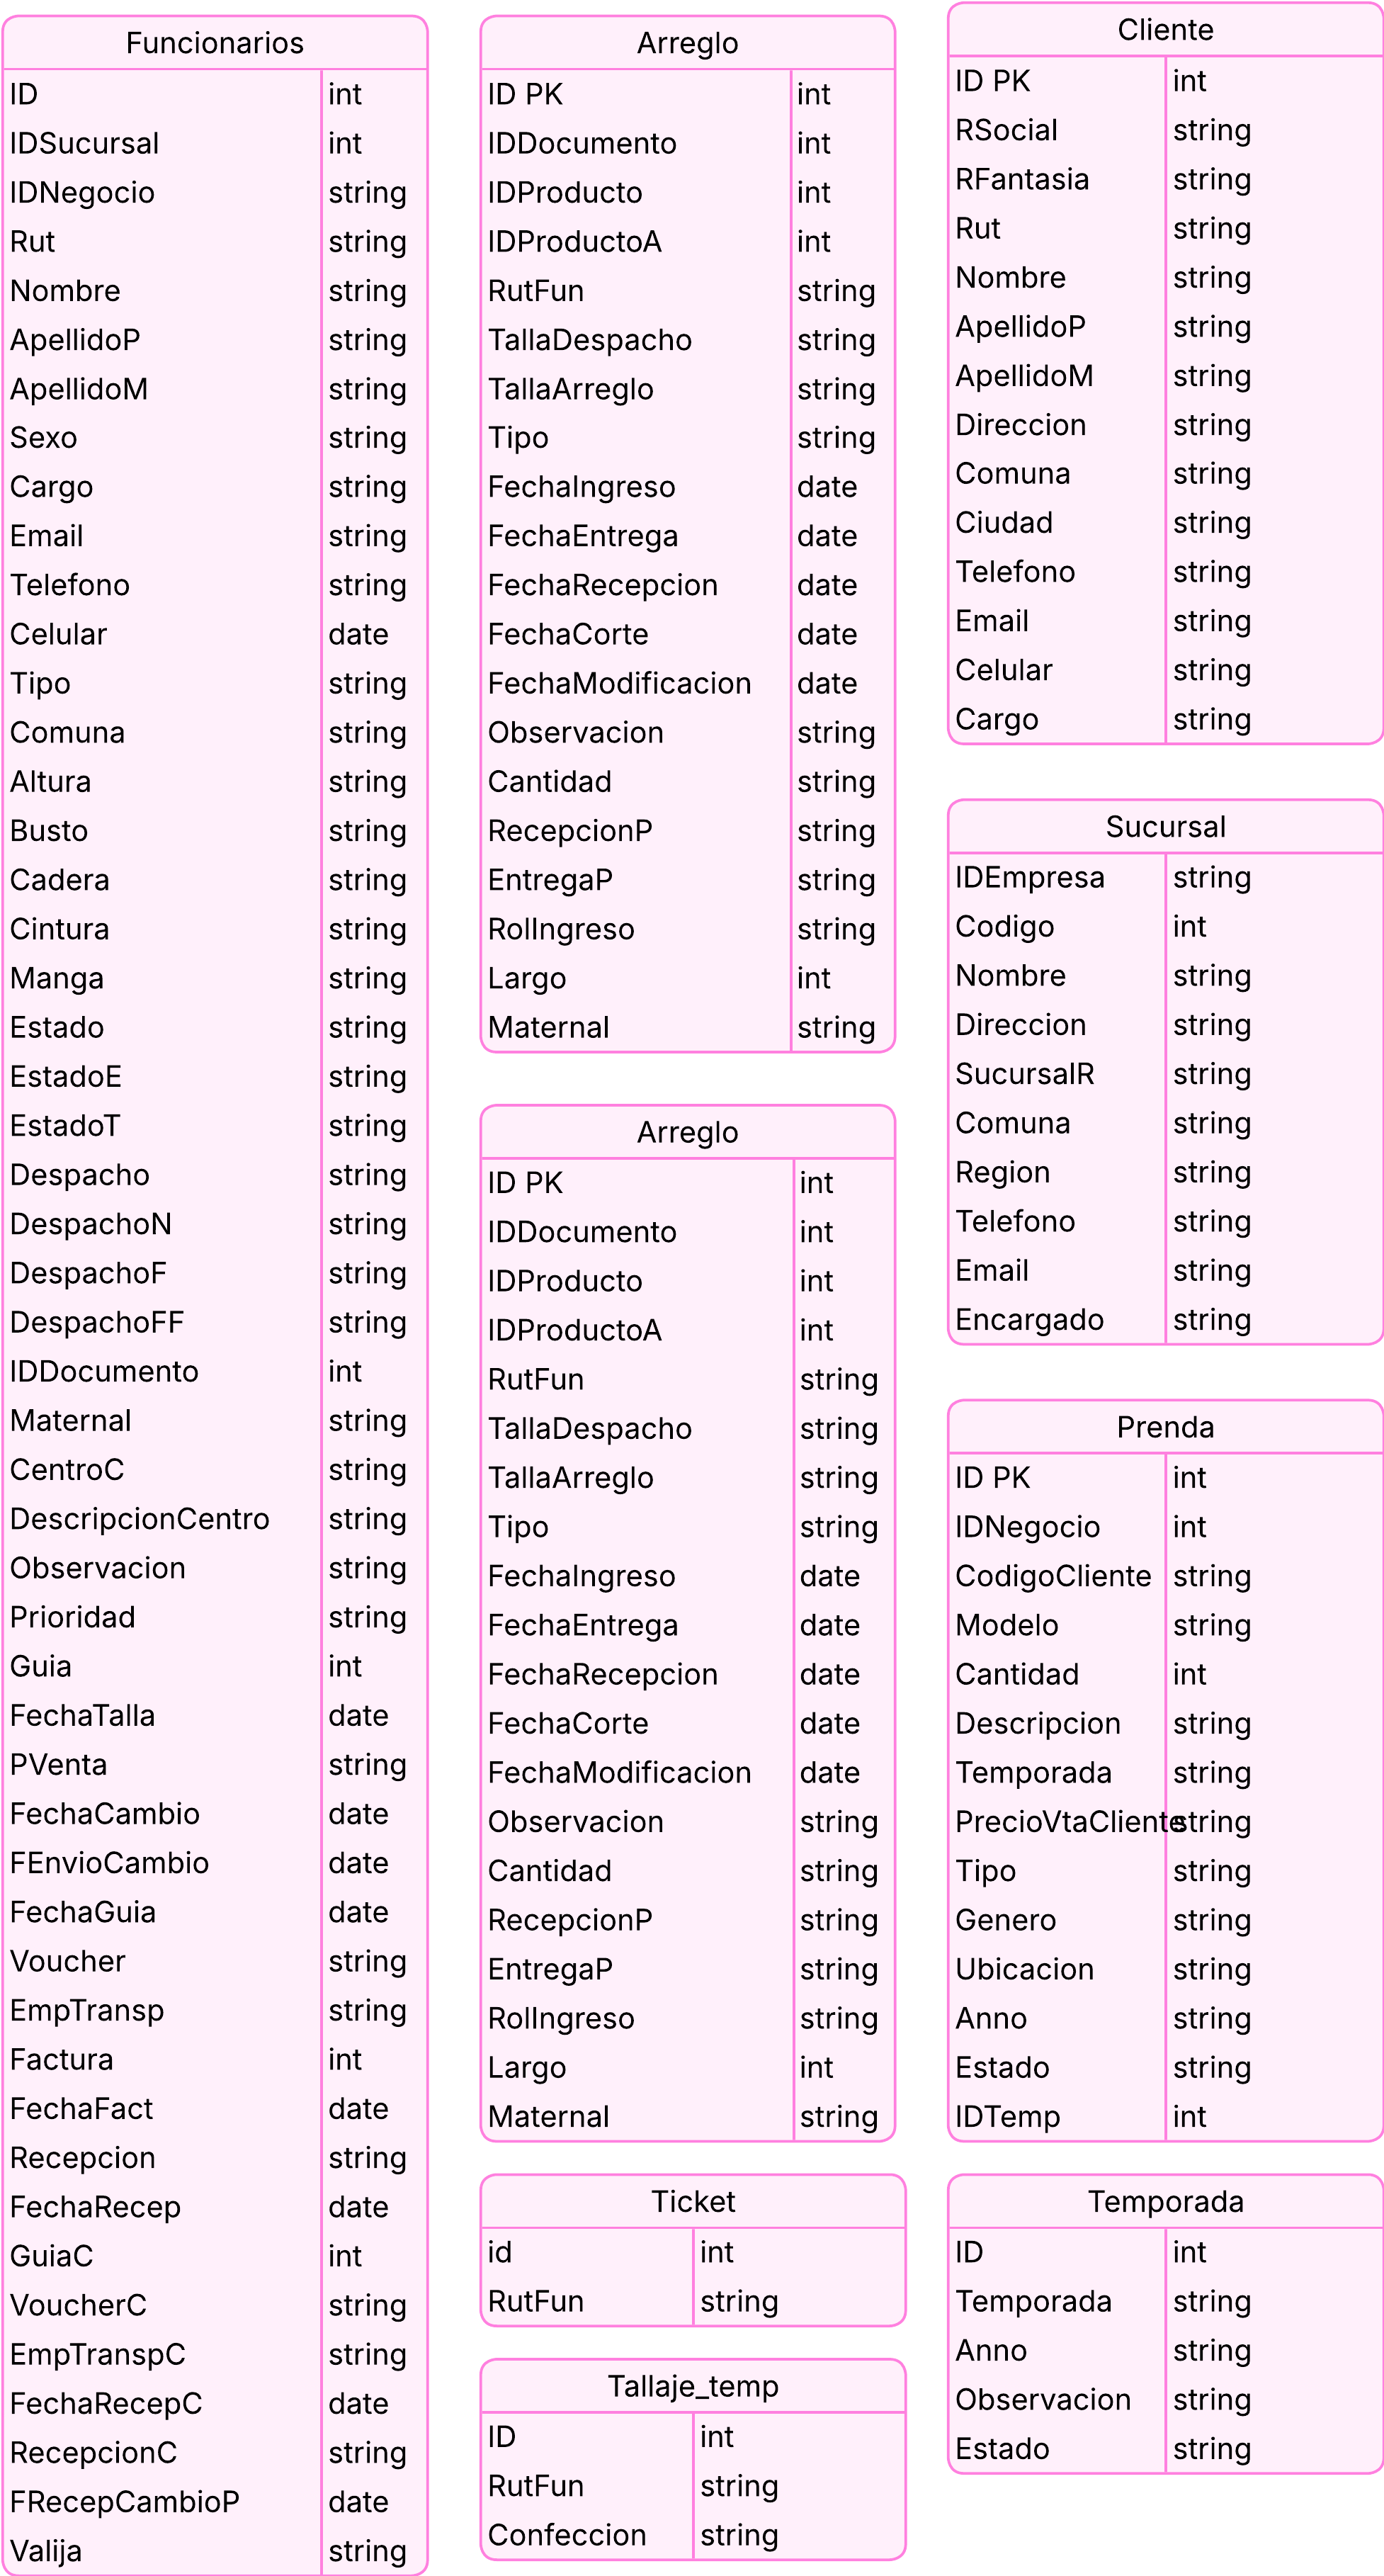
\includegraphics[height=0.9\textheight]{figuras/diagramas-actuales/diagrama-bdd-2}
    \caption{Diagrama físico de bases de datos del sistema actual (Parte 2)}
    \label{fig:diagrama-bdd-2-actual}
\end{figure}


\subsection{Diagrama de Flujo}

\subsection{Diagrama de Arquitectura}

\begin{figure}[htbp]
    \centering
    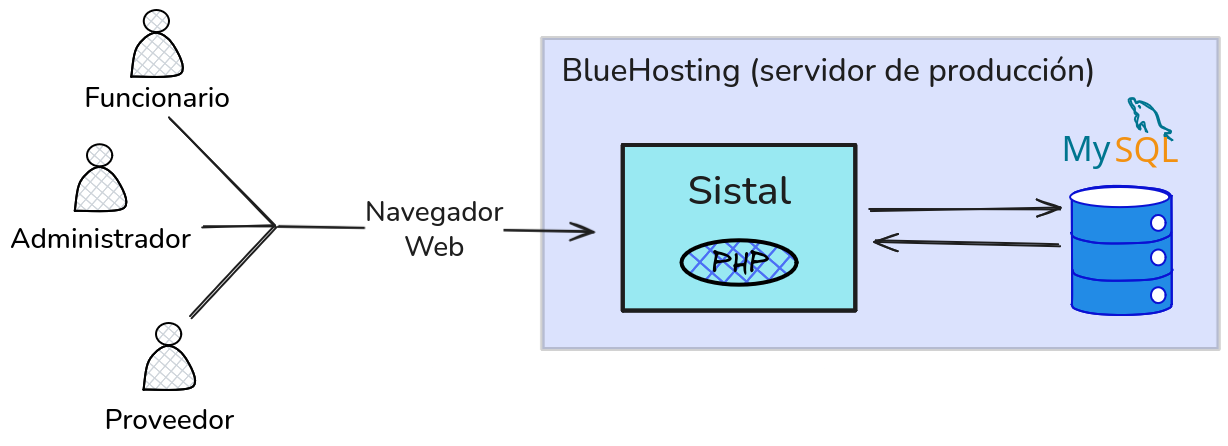
\includegraphics[width=\textwidth]{figuras/diagramas-actuales/diagrama-de-arquitectura}
    \caption{Diagrama de arquitectura del sistema actual}
    \label{fig:diagrama-arq-actual}
\end{figure}

\subsection{Diagrama de Despliegue}

\begin{figure}[htbp]
    \centering
    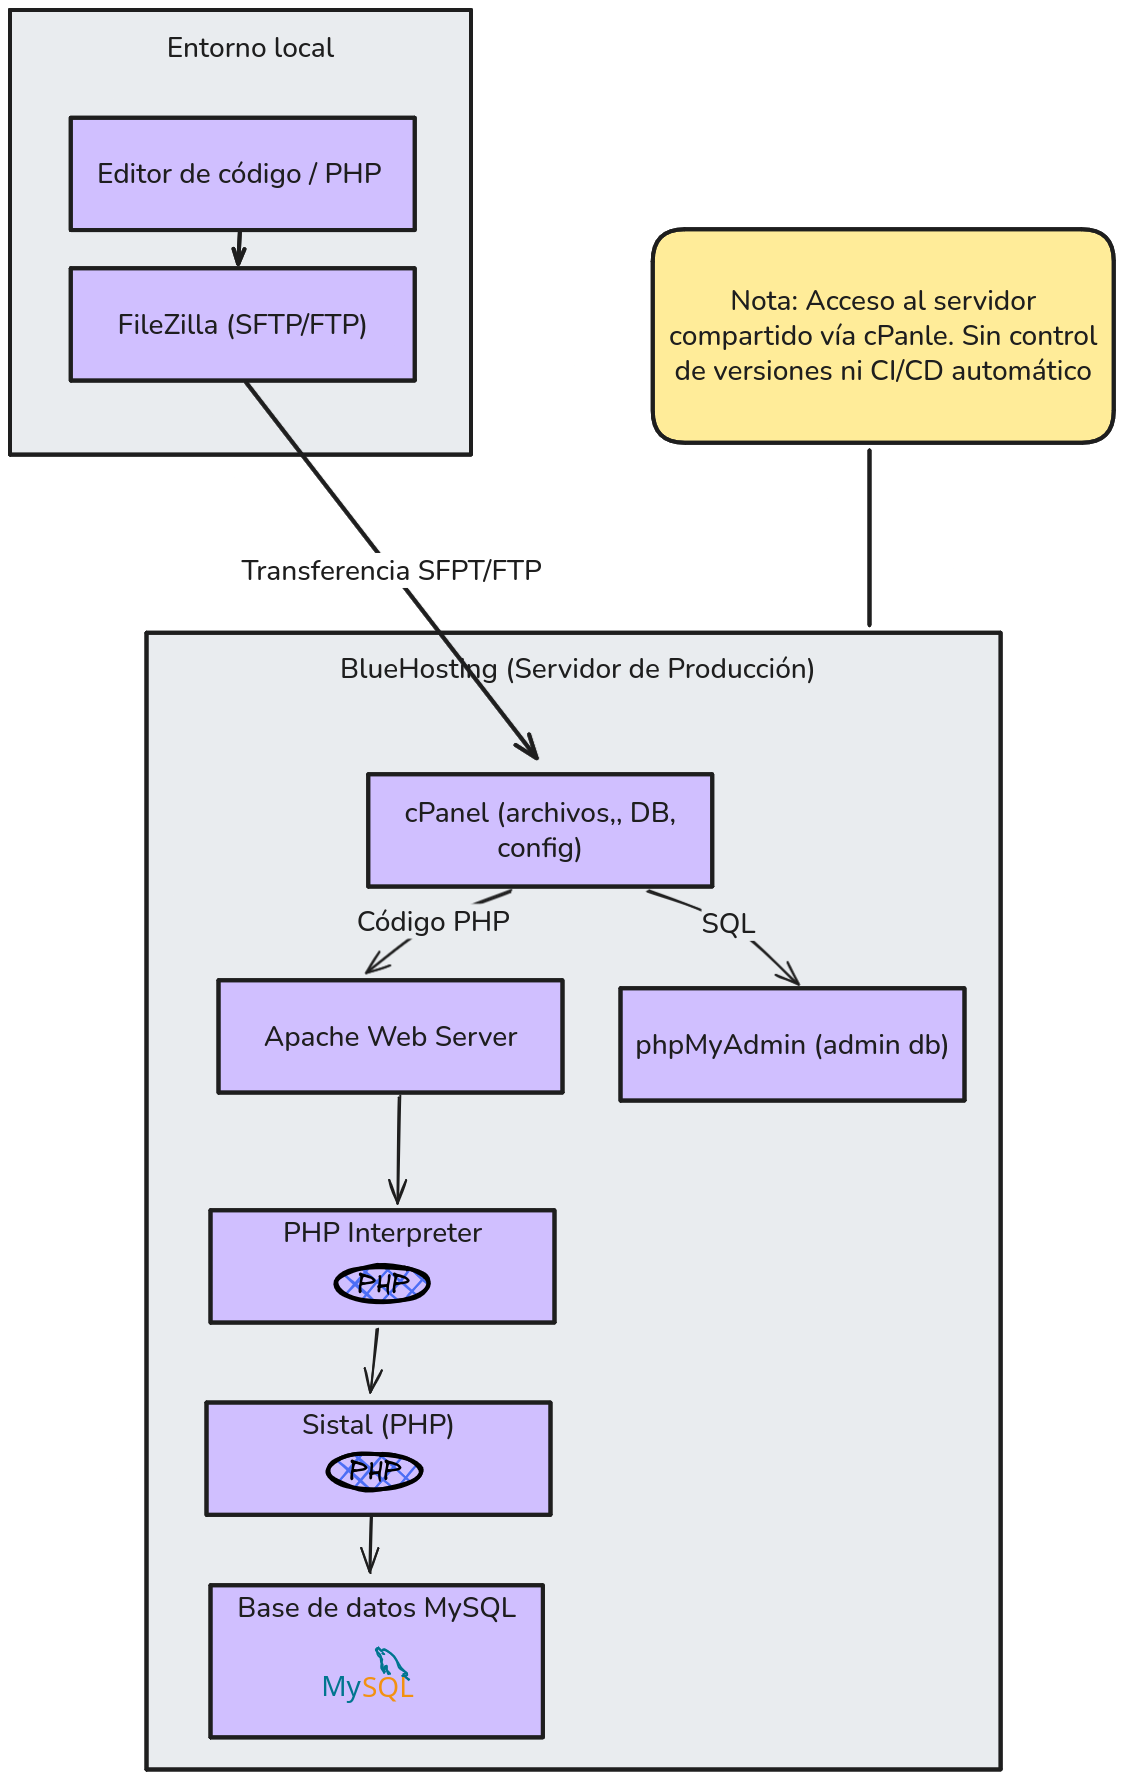
\includegraphics[width=0.8\textwidth]{figuras/diagramas-actuales/diagrama-de-despliegue}
    \caption{Diagrama de despliegue del sistema actual}
    \label{fig:diagrama-despliegue-actual}
\end{figure}

